\documentclass[11pt,a4paper]{article}
\usepackage[utf8]{inputenc}
\usepackage[T1]{fontenc}
\usepackage{graphicx}
\usepackage{hyperref}
\usepackage{geometry}
\usepackage{float}
\usepackage{booktabs}
\usepackage{longtable}
\usepackage{amsmath}
\usepackage{array}
\usepackage{xcolor}
\usepackage{enumitem}
\usepackage{microtype}
\usepackage[noblocks]{authblk}
\renewcommand\Affilfont{\small}
\geometry{a4paper, margin=0.85in}
\hypersetup{colorlinks=true, linkcolor=blue, urlcolor=blue, citecolor=blue}
\setlength{\parskip}{4pt}
\setlength{\parindent}{0pt}
\setlength{\emergencystretch}{3em}
% Long artifact paths are typeset in \texttt{} and contain no natural break
% points; allow the line breaker to split them rather than run into the margin.
\newcommand{\bs}{\discretionary{}{}{}}

\title{\textbf{Confidence Is Not Provenance: A Failure Analysis and Correction\\
of Cross-Layer Security-Evidence Fusion}}
\author[1,2,$\ast$]{Hardik}
\author[2,$\ast$]{Parth}
\affil[1]{Indian Institute of Technology Patna}
\affil[2]{Vivekananda Institute of Professional Studies -- Technical Campus (VIPS-TC), Delhi}
\affil[$\ast$]{These authors contributed equally and are joint first authors.}
\affil[ ]{\small Corresponding author: \texttt{hardikahlawat13@gmail.com}}
\date{8 September 2026}

\begin{document}
\maketitle

\begin{abstract}
Heterogeneous security evidence can be fused into a directed graph and ranked by path score. The confidence attached to a relationship, though, says nothing about whether evidence supports it. This paper is a failure analysis of our own prototype, AetherGraph, which fuses active reconnaissance, identity collection, repository secret scanning, web evidence and manual penetration-test findings, then ranks paths across those layers.

An earlier run, under the original semantics that walked every edge type, produced two cross-layer \emph{evidence} paths topping out at 0.914; under the corrected semantics neither qualifies as an attack path. Forensic reconstruction of the stored artifacts showed why. None of the relationships carrying that result had independent support in the collected evidence: the secret scanner emitted a fixed service target for every repository credential, the manual collector turned an analyst-supplied field straight into a graph relationship, and the identity collector built an account relationship out of an email address alone --- on a service provisioned for an entirely different user. The arithmetic was never at fault, and we reproduce the 0.914 figure exactly from the original streams. The defect lay in how the graph was constructed.

A second defect proved independent of the first. Path traversal treated every edge type as attacker movement, asset-containment and evidence-lineage relationships included. A three-node chain in the corrected graph, both of whose relationships are directly observed, scores 1.354 under that traversal --- above the unsupported path --- once the origin predicate is relaxed to the two origins the chain actually spans. That figure diagnoses the traversal defect rather than reporting a result: under the three-origin predicate used throughout the evaluation, the corrected graph yields no path under either traversal.

The corrected implementation labels every edge with its provenance (observed, derived, declared), requires a justification for anything derived, lets derivation rules decline when the evidence they need is missing, rejects edges into nodes no collector emitted, restricts attack traversal to capability relationships through an edge-semantics registry, and records controlled expectations for regression testing in a seed manifest. The corrected pipeline recovered all five expected relationships defined by that manifest and emitted neither of the two previously identified fabrication patterns. The corrected graph contains 14 nodes and 13 edges, of which 9 are observed, 3 derived and 1 declared, and contains no capability relationship. No valid attack path was produced under the defined access-edge traversal semantics, in any provenance mode.

A fresh live end-to-end execution against the running testbed reproduces this result: 9 observed, 3 derived and 1 declared relationship, no capability relationship, and no attack path. The evaluation remains confined to a controlled testbed containing no capability relationship of its own, so the zero-path outcome reflects that environment and supports no claim about others. A separate live positive control, run against a real Gitea instance with a verified access token and a working repository remote, confirms that the same rule emits a derived capability relationship when the required evidence is present, and that attack traversal then returns a non-empty path (score $0.855$). That is one controlled case, not a measure of accuracy or generality. The contribution is the documented failure mode and its remedy: confidence and provenance are orthogonal properties of a relationship, and a confidence value alone cannot distinguish an observation from an assumption.
\end{abstract}

\textbf{Keywords:} security knowledge graphs; evidence provenance; attack graphs; negative results; reproducibility; ablation; synthetic testbed

\section{Introduction}
Security assessment produces evidence in incompatible silos. A port scanner reports open services. An OSINT collector reports identities. A repository scanner reports leaked secrets. A penetration tester writes a report. Four artifacts, four formats, and nothing that ties them together.

Composition is where the risk lives. An open service may be routine; a leaked token may be inert. A leaked token that authenticates to that service is neither. Siloed tooling has no way to express that relationship, which is the standing argument for fusing evidence into one graph and ranking the paths through it. The idea is well established in the attack-graph literature, and it is the design AetherGraph implements.

The difficulty is that a fusion graph makes every relationship look alike. Once a scanner observation, a rule's inference and an analyst's assertion are all rendered as a typed arrow carrying a confidence value, nothing downstream can tell them apart. Confidence expresses how strongly a relationship is asserted; it says nothing about whether that relationship was observed, derived from evidence, or simply assumed. In our own prototype the consequence was concrete. We reported a high-scoring cross-layer path whose critical relationships were not conclusions drawn from evidence at all, but fixed constants sitting in the collector source.

This paper asks: \emph{what must be recorded about a relationship for a ranked path over fused security evidence to be interpretable as a security finding?} We approach it through a failure and its correction, with two objectives. The first is to work out why conventional safeguards --- confidence thresholds, path-length penalties, score reproduction, unit tests --- let unsupported relationships through. The second is to find the smallest construction discipline that keeps them out.

Our contributions are:
\begin{enumerate}[leftmargin=*]
\item A forensic analysis, reproduced from stored artifacts, demonstrating that confidence-weighted graph fusion can produce an apparently strong ranked result from relationships that are not independently supported by evidence, while every validation the system performed passes.
\item Identification of a second, independent defect: path traversal that treats asset-containment and evidence-lineage relationships as attacker movement, which we show can rank adequately supported evidence above the unsupported path.
\item A provenance-aware graph-construction mechanism distinguishing observed, derived and declared relationships, with mandatory justification for derived edges and endpoint validation that rejects edges into unemitted nodes.
\item Evidence-backed derivation rules that explicitly decline when required evidence is absent, and a semantic edge classification separating general evidence relationships from attack-traversable capability relationships.
\item A controlled regression methodology using expected and forbidden relationships to prevent recurrence of the identified fabrication patterns, evaluated by an ablation over collector layers, provenance levels and traversal semantics, which shows that the correction removes the previously reported high-scoring evidence path in this environment.
\item A live positive control establishing that the corrected derivation rule emits a capability relationship, and that attack traversal accepts it, when the required evidence genuinely exists --- so that the negative results are attributable to absent evidence rather than to a rule incapable of firing.
\end{enumerate}

\section{Related Work}
\textbf{Attack graphs and path ranking.} Automated attack-graph construction was established by Sheyner et al.\ using model checking to generate and analyze exploit sequences~[1], and by Ammann et al.\ with a monotonicity assumption that makes generation scale~[2]. MulVAL recast the problem in Datalog, deriving multi-host attack paths from configuration and vulnerability facts~[3]. Ingols et al.\ generated attack graphs for operational defensive use~[4]. Ranking is the closest sub-problem to this work: Mehta et al.\ ordered attack-graph states with a PageRank-style stationary distribution~[5], and Wang et al.\ combined per-vulnerability probabilities into a cumulative metric~[6]. Manadhata and Wing defined an attack-surface metric from entry and exit points, channels and untrusted data items~[7].

What unites that literature is an assumption about its inputs. Vulnerability and configuration facts arrive from a scanner or a database and are treated as given; the contribution is the reasoning performed over them. Our failure sits underneath that assumption, in the construction of the facts themselves, where no amount of rigour in the reasoning layer would have reached it.

\textbf{Security knowledge graphs.} The modern form of this idea is the cybersecurity knowledge graph, which fuses heterogeneous sources into one graph-based model to support threat intelligence, situational awareness and attack-path analysis; Sikos surveys the graph data models and knowledge-organisation systems involved~[17], and Zhao et al.\ survey construction techniques in detail, covering ontology design, entity recognition and relation extraction~[18]. Relation extraction is precisely where our problem lives. That literature is largely concerned with extracting \emph{more} relationships accurately from text and structured feeds; ours is a case where relationships were produced with no extraction step at all, by constants in collector source, and where the graph offered no way to tell the difference afterwards.

\textbf{Reconnaissance and OSINT automation.} Internet-scale scanning~[8] and general-purpose tooling such as Nmap~[9] underpin the active layer. Recent surveys catalog AI-assisted OSINT collection and asset discovery~[10,11], and Edwards et al.\ showed that an organization's social-engineering attack surface can be assembled automatically from public sources~[12]. Work in this area is generally evaluated on collection yield. The question we raise --- whether a relationship between two collected items is warranted --- is not usually posed.

\textbf{Evidence fusion, correlation and provenance.} Correlating vulnerability, asset and identity records into a single representation is long-standing practice, and separating an assertion's strength from its evidentiary origin is a familiar idea --- in data provenance, in structured threat-intelligence formats that carry confidence and source as distinct fields, and in provenance-based intrusion detection, where Zipperle et al.\ survey systems built specifically on the lineage of observed events~[19]. We claim no credit for that separation. Our narrower observation, which we support empirically rather than by appeal to the literature, is that graph-based security inference requires the distinction to be enforced \emph{per edge and at construction time}, because path scoring multiplies edge values together and thereby aggregates assumptions and measurements into a single number with no residual trace of which was which. We are not aware of prior work that reports this specific failure mode in a fusion pipeline, but we make no priority claim: our contribution is the documented failure, its diagnosis and a construction discipline, not the concept of provenance.

\textbf{Tooling and standards.} The prototype is built on NetworkX for graph storage and traversal~[13]. Its manual layer follows the structure practitioners already use --- the OWASP Web Security Testing Guide~[14] and the Penetration Testing Execution Standard~[15] --- and DVWA~[16] is one of the four services in the testbed. These are instruments rather than related work, but what the pipeline is able to observe depends on them, so they belong on the record.

\textbf{Evaluation practice.} Our evaluation is a controlled testbed study, and the limits of that design are themselves an active concern in adjacent work. Happe and Cito, reviewing benchmarking practice across nineteen studies in LLM-driven offensive security, find that conclusions depend heavily on testbed choice, that baselines are frequently absent, and that constructed challenges often fail to represent real engagements~[20]. We read our own evaluation the same way, and Section~\ref{sec:eval} states its scope in those terms rather than leaving a reader to infer it.

\textbf{Distinguishing this work.} We propose neither a new attack-graph formalism nor an improved risk metric, and we claim no novelty for provenance as a concept. What we report is a construction-time failure mode in a fusion pipeline, evidence that conventional safeguards did not detect it, and an architectural change that stops the identified patterns recurring. The result is a controlled negative one on a single synthetic testbed --- not a performance claim.

\section{System and Architecture}
\subsection{Synthetic Testbed}
The testbed is a four-container Docker Compose environment: Nginx on port 80, vsftpd on 21, Gitea on 3000 and DVWA on 8080. Into it we planted an email address in an HTML comment, a plaintext credential file behind a directory-listing-enabled path, an exposed \texttt{.git/config} naming a repository owner, an invalid AWS-shaped canary committed to a local repository, and a single-row breach corpus. A hand-authored report contributes two manual findings. The FTP container is provisioned with \texttt{FTP\_USER=test}, a detail that matters in Section~\ref{sec:baseline}.

Everything in the environment was placed there deliberately. This is what makes the controlled expectations of Section~\ref{sec:groundtruth} available without an external labelling effort, and equally what prevents any result obtained here from generalizing beyond it.

\subsection{Collectors and Common Schema}
Six collectors emit JSON Lines in a uniform record shape: an identifier, an attribute object, and zero or more outgoing edges. Fusion happens through identifier equality alone --- there is no entity resolution --- so two collectors agree about an entity exactly when they emit the same identifier string.

The active collector runs Nmap and Gobuster in Docker. A web-evidence collector retrieves the content behind discovered paths and probes for exposed Git configurations. An identity collector harvests addresses from the target's HTML and checks them against the local corpus. A secret scanner walks committed revisions for canary patterns. A manual collector ingests the structured report. A Nuclei collector runs a bounded, digest-pinned scan.

Every record carries an \texttt{origin} of \texttt{active}, \texttt{identity} or \texttt{manual}, which is what the cross-layer predicate is defined against. Table~\ref{tab:nodes} lists the node types the implementation exercises.

\begin{table}[H]
\centering
\caption{Node types and the attributes the collectors populate.}
\label{tab:nodes}
\small
\begin{tabular}{p{0.20\textwidth}p{0.70\textwidth}}
\toprule
Type & Attributes used \\
\midrule
Host & IP address, asset class, origin \\
Service & Port, protocol, service name, product, version, severity, asset class, origin \\
WebPath & Path, HTTP status, severity, origin \\
Exposure & Kind, source URL, parsed fields (email, repository name), severity, origin \\
Persona & Email, origin \\
Credential & Source, severity, secret kind, commit/file or source URL, origin \\
Account & Username, severity, origin \\
Finding & Class, title, location, severity, CVSS base, evidence references, origin \\
\bottomrule
\end{tabular}
\end{table}

\subsection{Edge Provenance}\label{sec:provenance}
Every edge carries a provenance label. The three levels are deliberately coarse and mutually exclusive:

\begin{itemize}[leftmargin=*]
\item \textbf{Observed.} A tool reported the relationship directly, with no inference step. Nmap saw the service on the host; a fetched file contained a credential pair.
\item \textbf{Derived.} A deterministic rule combined two or more observations and recorded a justification naming the evidence. The defining property is that a derivation rule must be able to \emph{decline}: absent evidence yields no edge.
\item \textbf{Declared.} A human asserted the relationship in a report. It may be true, but it entered the graph because someone wrote it down.
\end{itemize}

Provenance is mandatory: the edge constructor rejects an edge without it, and rejects a derived edge with no justification.

The three levels are an operational taxonomy, chosen for this prototype to keep direct observation, deterministic evidence-based derivation and explicit human assertion apart. We do not claim it is theoretically complete, minimal, or universally correct. Finer distinctions are plainly available --- between tool classes of differing reliability, say, or between derivation rules of differing strength. This is a design choice that served the failure analysed here, and it would need broader validation before anyone recommended it generally.

One loading rule follows from the same caution. A stream written before provenance labelling existed loads as \emph{declared}, the most conservative reading available, so a legacy artifact can be compared against without being quietly promoted to discovered.

\subsection{Terminology}\label{sec:terminology}
Because the distinction is central to every result reported here, we fix three terms.

\begin{description}[leftmargin=*,style=nextline]
\item[Evidence graph] The directed graph representing relationships among collected observations. All edges of all semantic categories belong to it. It is the artifact the collectors produce.
\item[Attack (capability) traversal] A restricted traversal over only those edge types whose semantics represent attacker capability or movement. A path returned by this traversal is termed an \emph{attack path}, and this is the only traversal whose output may be so described.
\item[Evidence traversal] An unrestricted traversal over all edge types. Its output is termed an \emph{evidence path}. It is a diagnostic device --- useful for reproducing the pre-correction behaviour and for inspecting connectivity --- and must not be interpreted as exploitation or attacker movement.
\end{description}

Throughout, a directed path in the evidence graph is not an attack path merely by virtue of being a path. The chain \texttt{credential} $\rightarrow$ \texttt{web path} $\rightarrow$ \texttt{service} is an evidence path; \texttt{service} $\rightarrow$ \texttt{host} records asset containment and is not attacker movement in either direction. We classify edges by what they assert rather than reversing them to suit a traversal, so edge directions in this schema remain heterogeneous by design; Section~\ref{sec:discussion} returns to this as a limitation.

\subsection{Edge Semantics}\label{sec:semantics}
Provenance answers how we know an edge exists. It does not answer what the edge asserts, and path traversal depends on the latter. We therefore classify every edge type into one of five semantic categories, shown in Table~\ref{tab:semantics}. An edge type absent from the registry is rejected at load time rather than given a default, so a new collector cannot quietly introduce a relationship whose meaning nobody has decided.

\begin{table}[H]
\centering
\caption{Edge types, their semantics, and eligibility for attack-path traversal.
Only capability relationships describe attacker movement.}
\label{tab:semantics}
\small
\begin{tabular}{p{0.20\textwidth}p{0.14\textwidth}p{0.41\textwidth}c}
\toprule
Edge type & Category & Assertion & Traversable \\
\midrule
HOSTS\_SERVICE & containment & service runs on host & no \\
SERVES\_PATH & containment & service serves web path & no \\
EXPOSED\_BY & evidence & fact was retrieved from location & no \\
IDENTIFIES & evidence & exposure names a persona & no \\
EXPOSES\_\bs CREDENTIAL & evidence & corpus row matches a persona & no \\
VALIDATES & validation & analyst tested this asset & no \\
CORRELATES & correlation & asserted association, no mechanism & no \\
OWNS\_ACCOUNT & access & persona controls account & \textbf{yes} \\
ENABLES\_ACCESS & access & credential authenticates to service & \textbf{yes} \\
\bottomrule
\end{tabular}
\end{table}

Only \emph{access} edges are walked when inferring an attack path, in the sense fixed in Section~\ref{sec:terminology} --- that is, $\mathit{ATTACK\_TRAVERSABLE} = \{\textsc{access}\}$. This is an operational definition for this prototype and a controlled design decision, not a claimed universal ontology of attack relationships. Assigning nine edge types to five categories reflects our judgement about this schema, and nothing outside this paper has validated it. Widening the traversable set is a research decision that needs an argument behind it, not a convenience.

Traversing the full evidence graph remains possible, because evidence-graph connectivity is a legitimate question in its own right. It is simply a different question, and Section~\ref{sec:eval} keeps the two answers apart.

\subsection{Derivation Rules and Graph Construction}
Four rules produce derived edges, each stated as a conjunction so that a missing conjunct yields nothing:

\begin{enumerate}[leftmargin=*]
\item \textbf{Repository secret to service.} Requires a repository remote identifying a concrete service, that service having been independently observed, and the secret's kind being compatible with the observed product.
\item \textbf{Persona to account to service.} Requires corroborating evidence naming both the username and a specific observed service. A harvested email address is not corroboration that an account exists.
\item \textbf{Finding to service.} Parses the \texttt{location} the analyst recorded and matches it against observed services. Host equivalence must be declared explicitly by the operator; port agreement alone is not a match, and an ambiguous match is declined.
\item \textbf{Exposed content to persona.} An exposed \texttt{.git/config} recording a \texttt{user.email} identifies a persona.
\end{enumerate}

Rules record why they declined, which is reported at run time and is how a reader tells ``no relationship exists'' apart from ``the collector was silent''.

Graph construction loads all nodes from all streams before any edge, then validates both endpoints of every edge. An edge referencing a node that no collector emitted is refused with an error naming the offending stream. This suppresses the default NetworkX behaviour of materialising a missing endpoint as an attribute-less node, which would otherwise enter scoring with no type, no origin and severity zero.

\section{Path Scoring}\label{sec:scoring}
For a node $v$ the implementation computes
\begin{equation}
CR(v)=0.40\,S(v)+0.25\,R(v)+0.25\,B(v)+0.10\,A(v),\label{eq:cr}
\end{equation}
where $S(v)$ is stored severity, $R(v)=1/(1+d(v))$ with $d$ the shortest directed distance from any entry node ($d=99$ when unreachable), $B(v)$ is the fraction of designated jewel nodes reachable from $v$, and $A(v)$ is an asset-class weight. For a simple path $\pi$,
\begin{equation}
P(\pi)=\left(\prod_{e\in\pi}c(e)\right)\left(\sum_{v\in\pi}S(v)\right)\lambda^{|\pi|-1},\qquad \lambda=0.95.\label{eq:path}
\end{equation}

Both equations were checked against the implementation. The weights are fixed in source as stated, $\lambda=0.95$, and the confidence floor of $0.60$ rejects any edge beneath it. Note that $|\pi|$ counts \emph{nodes}, so a length bound of 5 admits at most 4 edges. Severity absent from a record and severity present but explicitly null both normalise to $0.0$; the second case used to raise a type error and now has a regression test on it.

Two conventions deserve naming rather than burying. Entry nodes are those of identity or manual origin, and jewels are service records. Both are conventions of the runner, not a validated organisational asset model.

\textbf{What a path means, and what it does not.} A returned path asserts that a chain of capability relationships exists between recorded entities, each above the confidence floor, and that the chain spans the required evidence origins. It does not assert that the chain is exploitable, that any credential was tested, or that an attacker could traverse it. It is a ranked hypothesis for an analyst to examine, and its value depends entirely on the provenance of the edges composing it --- which is the subject of the next section.

\section{Baseline and Failure Analysis}\label{sec:baseline}
\subsection{The Original Result}
The original run is stored under \texttt{out/\bs integrated\bs \_experiment\bs \_20260824\bs \_000517}: 13 nodes, 13 edges, and two paths satisfying the active--identity--manual predicate under evidence traversal, the semantics the implementation then used. The highest-scoring path had a score of 0.914:
\begin{verbatim}
finding-MAN-DVWA-LOGIN -> cred-git-1 -> svc-192.168.65.254-3000
\end{verbatim}
Loading those stored streams and rescoring them reproduces both paths and both scores exactly, 0.914 and 0.868. By Equation~\eqref{eq:path}, with edge confidences $0.75$ and $0.75$, severities $0.6$, $0.9$ and $0.3$, and discount $0.95^{2}$: $0.5625\times1.8\times0.9025=0.914$. The scoring computation is therefore internally consistent and exactly reproducible from the stored artifacts.

\subsection{Forensic Reconstruction}
Reading the collector source, rather than only its output, established that the relationships carrying that path had no independent support in the collected evidence. Three distinct generation mechanisms were responsible; two of them appear in the highest-scoring path itself.

\textbf{The \texttt{ENABLES\_ACCESS} edge.} For every credential found in any repository, the secret scanner emitted an edge to \texttt{svc-\{ip\}-3000}. The port was a literal in the source, so nothing about the credential, the repository or the observed environment took part in choosing it. In practice this meant an AWS-shaped canary was linked to a Gitea service --- unrelated technologies --- from a seed repository that has no configured remote at all.

\textbf{The \texttt{CORRELATES} edge.} The manual report carried a \texttt{related\_credentials} field which the collector converted directly into a graph relationship with no evidentiary check. The identifier \texttt{cred-git-1} was supplied by the analyst in the input file, and the pipeline subsequently ranked the path containing it. The relationship was therefore declared rather than discovered, and the evaluation was to that extent circular.

\textbf{A third mechanism.} The identity collector created \texttt{account-\{user\}-ftp} for every harvested email address and linked it to port 21 unconditionally, with no verification that the account existed. The FTP container is provisioned with \texttt{FTP\_USER=test}, so the node corresponded to no entity in the environment. This relationship did not appear in the highest-scoring path but was present in the graph.

Figure~\ref{fig:baseline} shows the baseline graph with both unsupported relationships marked. We use the term \emph{fabrication pattern} in the remainder of the paper as a shorthand for a relationship generated without evidentiary support by one of these mechanisms; it denotes a defect in construction, not an allegation of intent.

\begin{figure}[H]
\centering
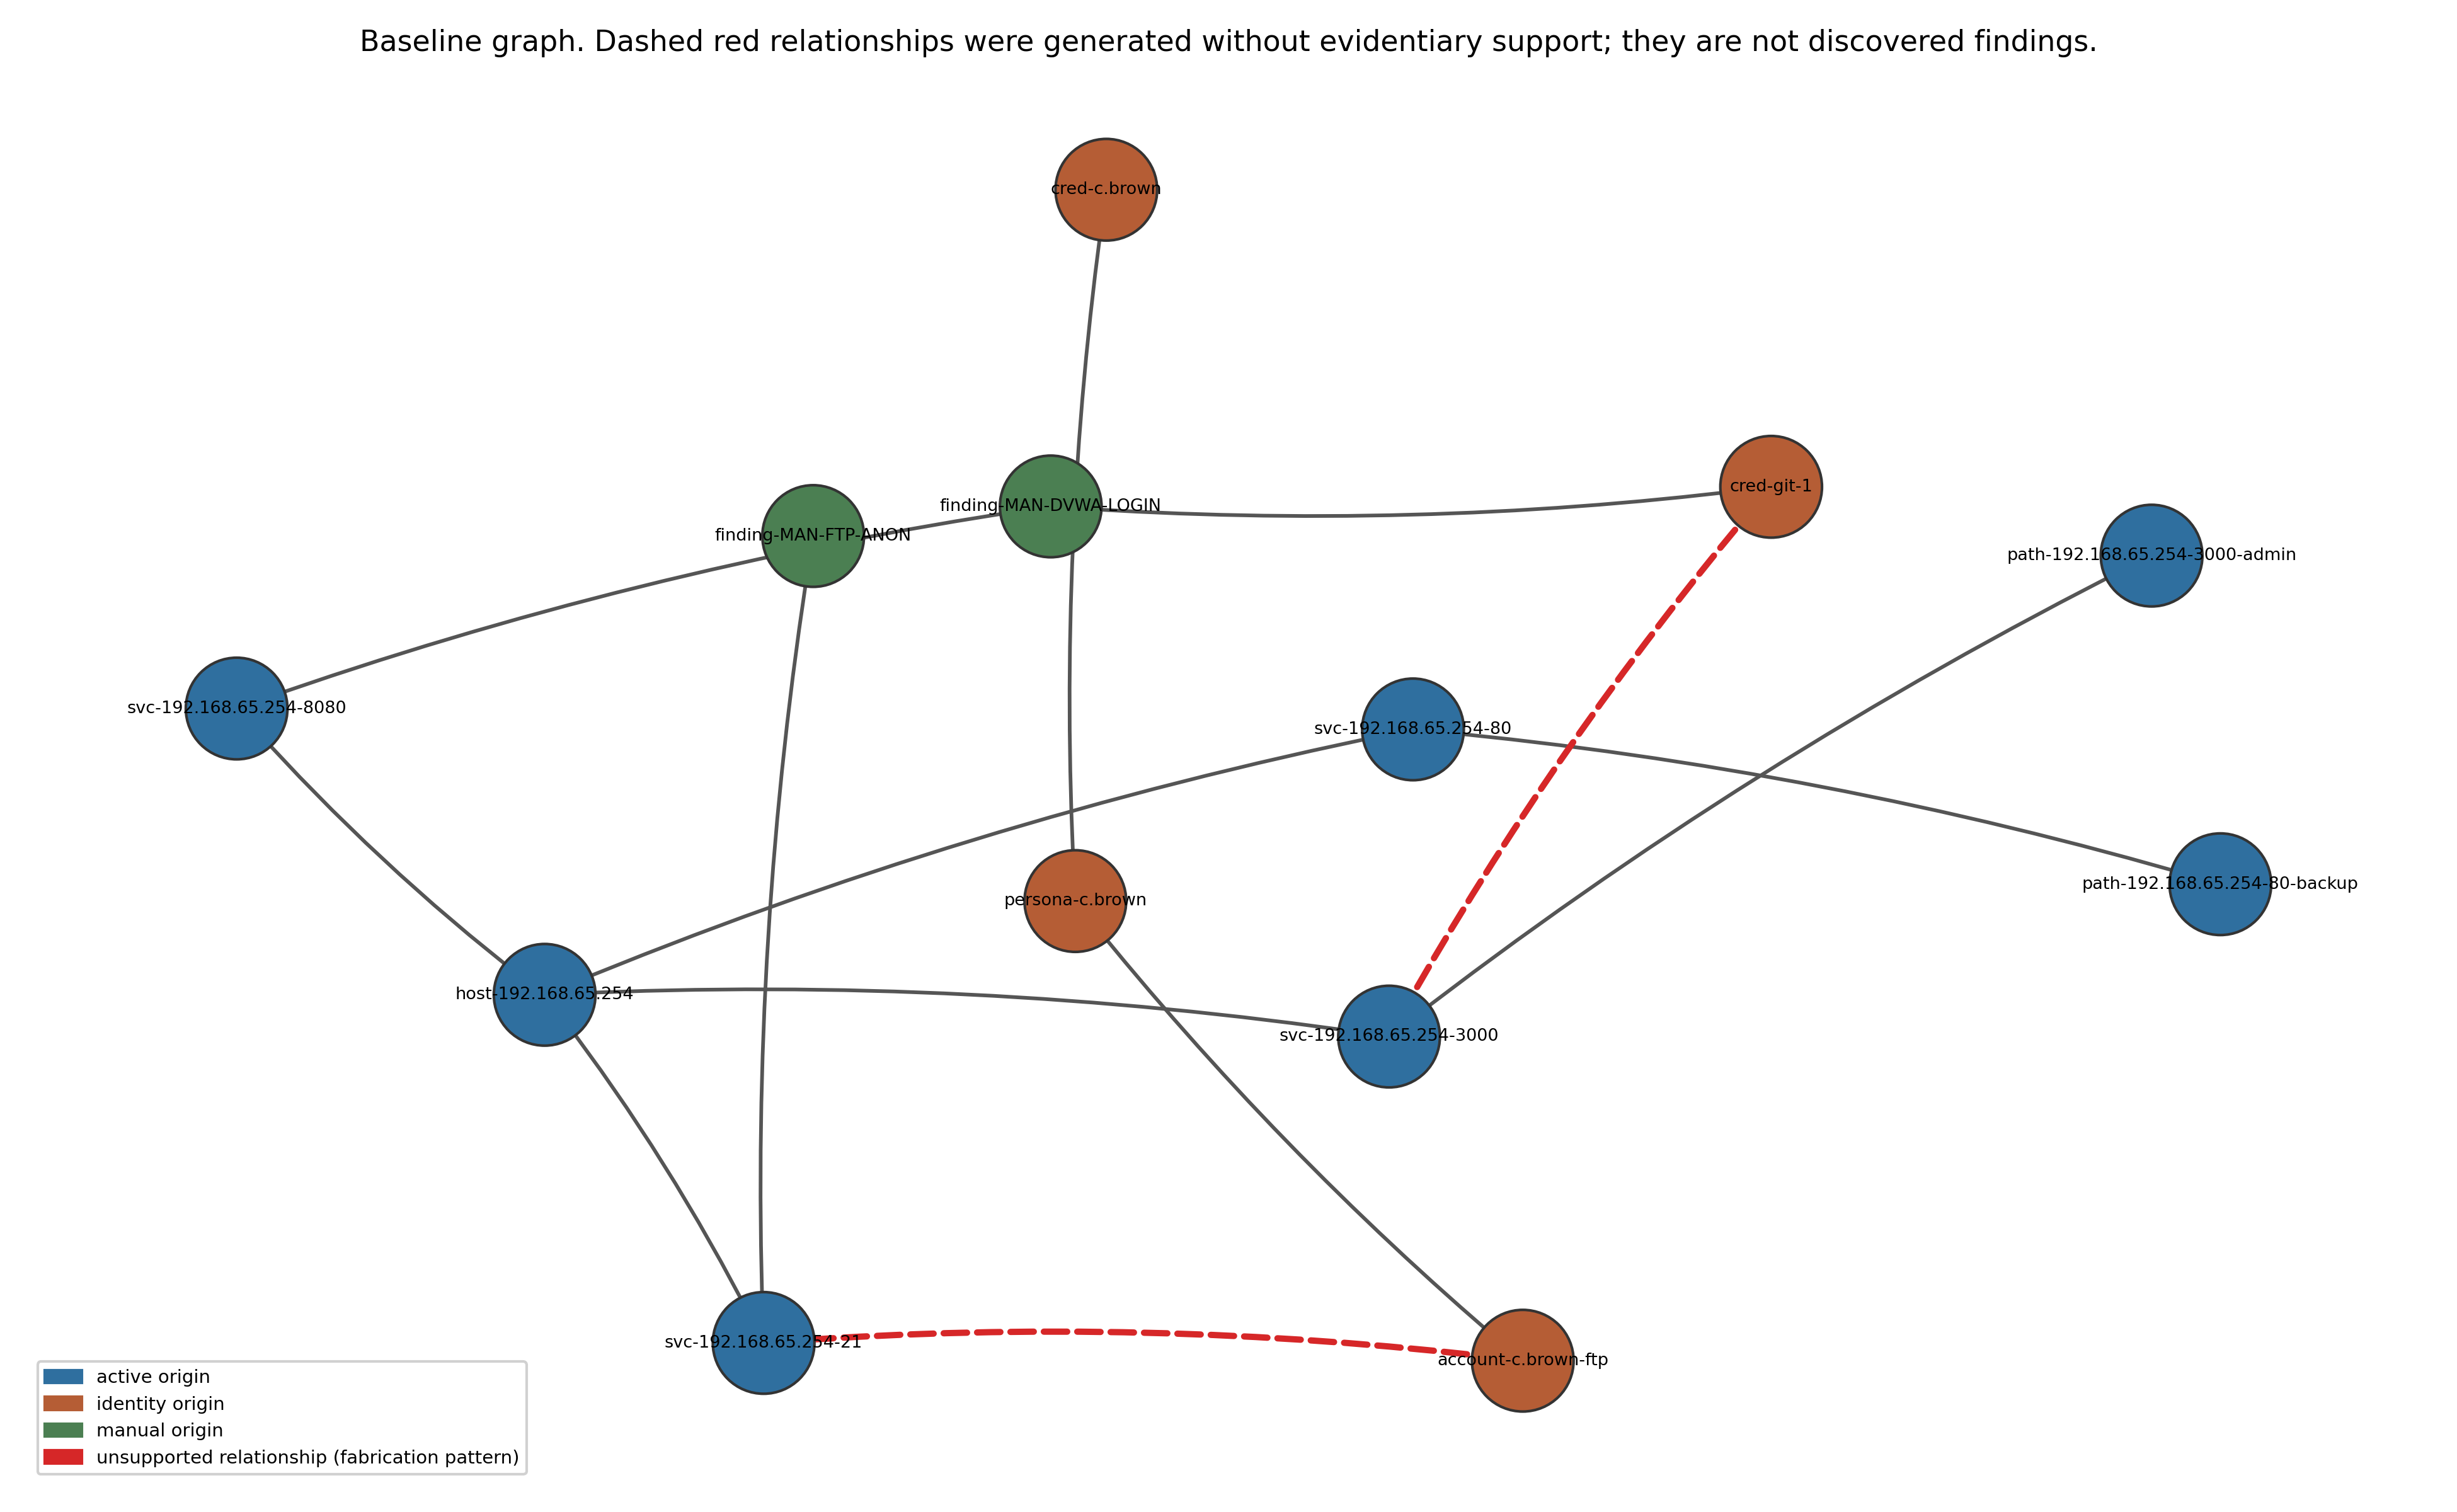
\includegraphics[width=0.95\textwidth]{out/derived_experiment_20260908/Figure_baseline_graph.png}
\caption{The baseline graph rebuilt from its stored artifacts. Dashed red edges are the
hardcoded relationships identified by the forensic reconstruction; they were not derived
from evidence. Node colour indicates recorded origin.}
\label{fig:baseline}
\end{figure}

\subsection{Why the Existing Safeguards Did Not Detect It}
Every check the system performed was satisfied by that path. Both unsupported edges exceeded the $0.60$ confidence floor at $0.75$. The length penalty applied normally. The cross-layer predicate held. Rescoring reproduced the result to three decimal places. All eight unit tests then present passed, and one of them asserted the defective behaviour as expected output, which had the effect of protecting the defect from change.

The common cause is straightforward once stated. Every check asked how strongly a relationship was asserted; none asked where it came from. A confidence of $0.75$ assigned by a scanner and a confidence of $0.75$ typed by a human are indistinguishable to everything downstream, and Equation~\eqref{eq:path} multiplies them together without distinction.

\subsection{A Second, Independent Defect}
Correcting provenance alone would not have been sufficient. The original traversal walked every edge type as though it were attacker movement. Consider a chain drawn entirely from the corrected graph, in which every edge is observed and correctly justified:
\begin{verbatim}
cred-web-1 --EXPOSED_BY--> path-80-backup --SERVES_PATH--> svc-80
\end{verbatim}
These relationships state that a credential was retrieved from a URL and that a service serves that path. Neither asserts a capability.

The status of this chain deserves precision. Both of its relationships are directly observed, and the chain genuinely sits in the corrected graph of Section~\ref{sec:eval}; it is not a hypothetical construction. It does not appear among the reported results because every configuration in this paper requires a path to span all three evidence origins, and this chain spans two (identity and active). Relaxing the predicate to those two origins and traversing all edge types --- the semantics the pre-correction implementation used --- the chain and its extensions score 1.354, 1.286 and 1.14, each exceeding the 0.914 of the unsupported path. The figures are reproducible from the recorded artifacts via \href{scripts/verify_evidence_chain.py}{\texttt{scripts/verify\_evidence\_chain.py}}.

The consequence is that adequately supported evidence, traversed under inappropriate semantics, outranks an unsupported relationship. Provenance alone would therefore not have been sufficient.

This is why Section~\ref{sec:semantics} classifies edges by what they assert. The two defects are independent: provenance prevents unwarranted relationships from entering the graph, and semantics prevents warranted relationships from being read as something they are not.

\section{Corrected Architecture}\label{sec:corrected}
The correction comprises five changes, each targeting a specific finding above. The scoring of Section~\ref{sec:scoring} is unchanged: the arithmetic was never at fault.

\textbf{Provenance with mandatory justification.} Every edge is labelled observed, derived or declared. The constructor rejects a missing or unknown provenance, and rejects a derived edge carrying no justification string.

\textbf{Derivation rules that decline.} The three fabrications are replaced by the rules of Section~\ref{sec:provenance}. On the current testbed all three decline: the secret scanner reports \emph{0 of 1} findings with an evidence-derived service link, and the identity collector reports \emph{1 persona with no account link}, both printed at run time.

\textbf{Endpoint validation.} Edges into nodes no collector emitted are refused. This was not hypothetical: the web-evidence collector emits an \texttt{IDENTIFIES} edge to a persona produced by a different collector, and when we introduced the check it immediately failed an ablation cell that withheld the identity stream. That cell had previously been reporting a phantom node in its totals. Ablations now drop such edges and report the count; the complete run is loaded strictly.

\textbf{Edge semantics.} Attack traversal is restricted to capability relationships per Table~\ref{tab:semantics}.

\textbf{Declared relationships stay declared.} The analyst's asserted correlation is retained, labelled declared, excluded from the derived-only graph, and never eligible for attack traversal. We do not reinterpret it as a discovery.

One design consequence is worth recording. The manual report previously carried a field naming the target service directly, which let the analyst address graph nodes. It now records only where the analyst tested, and a rule matches that against observed services. This is a weaker demand on the analyst and a stronger piece of evidence. Because the analyst reaches the testbed on a published loopback address while the scanner records the Docker gateway address, the host equivalence must be declared explicitly by the operator; without it the rule declines rather than matching on port number alone.

\section{Experimental Evaluation}\label{sec:eval}
\subsection{Controlled Expectations and the Limits of This Evaluation}\label{sec:groundtruth}
\texttt{testbed/seed\_manifest.json} records five \emph{expected} relationships, each with the node-identifier pattern and the provenance level a correct pipeline should produce, and two \emph{forbidden} relationships naming the fabrication patterns of Section~\ref{sec:baseline} together with the source construct responsible for each. The forbidden entries are retained as permanent regression tests.

The corrected pipeline recovered all five expected relationships defined by the manifest and emitted neither of the two forbidden patterns.

\textbf{This is a controlled regression check, not a recall measurement.} We state the circularity explicitly rather than leave it for a reader to infer. We constructed the testbed, we planted the evidence, we authored the derivation rules, and we then wrote the manifest that specifies what those rules should recover. The manifest therefore defines controlled expectations against which the implementation is regression-tested; it does not constitute independent ground truth, and the ``five of five'' figure must not be read as a recall statistic, as an estimate of detection performance, or as evidence of generality. Its evidential value is narrow and specific: it establishes that the two identified fabrication patterns do not recur, and that the replacement rules still emit the relationships the environment was built to contain.

A related circularity affects the manual layer and is likewise scoped rather than resolved. The penetration-test report is human-authored, and the analyst's asserted correlation remains in the graph as a declared relationship. We do not count it as a discovery, do not admit it to attack traversal, and exclude it from the derived-only configuration.

\subsection{Baseline versus Corrected}
Table~\ref{tab:compare} compares the two graphs under both traversal semantics, with the corrected architecture of Section~\ref{sec:corrected} applied to the rebuilt run. Table~\ref{tab:ledger} maps every claim in this paper to the artifact supporting it, and Appendix~\ref{app:refs} lists the works cited.

\begin{table}[H]
\centering
\caption{Baseline and corrected graphs. Evidence traversal walks every edge type, as the
original implementation did; attack traversal walks only capability edges. The baseline
figures are reproduced from the original stored artifacts and do not constitute a correct reference.}
\label{tab:compare}
\small
\begin{tabular}{lcc}
\toprule
 & Baseline & Corrected \\
\midrule
Nodes & 13 & 14 \\
Edges & 13 & 13 \\
Observed / derived / declared & 0 / 0 / 13 & 9 / 3 / 1 \\
Capability (access) edges & 3 & 0 \\
Fabricated relationships present & 2 & 0 \\
Cross-layer paths, evidence traversal & 2 (top 0.914) & 0 \\
Cross-layer paths, attack traversal & 0 & 0 \\
\bottomrule
\end{tabular}
\end{table}

Three things follow from that table. First, the baseline's edges carry no provenance annotation at all and so load as declared --- the most conservative reading of an unlabelled artifact, rather than a claim about what its authors intended. Second, the baseline yields no valid attack path under access-edge traversal semantics even with its unsupported edges intact, because the first relationship in its highest-scoring path is an asserted correlation, which does not represent attacker capability. The original result is therefore invalid on two independent grounds: the relationships were not evidence-supported, and the traversal semantics under which it was produced were inappropriate. Third, the corrected graph contains no capability relationship, which is the immediate reason its attack-traversal count is zero. We note this plainly: the corrected system did not discover an attack, and the present testbed offers it no opportunity to do so.

Figure~\ref{fig:corrected} shows the corrected graph coloured by provenance, and Figure~\ref{fig:counts} the record counts by origin.

\begin{figure}[H]
\centering
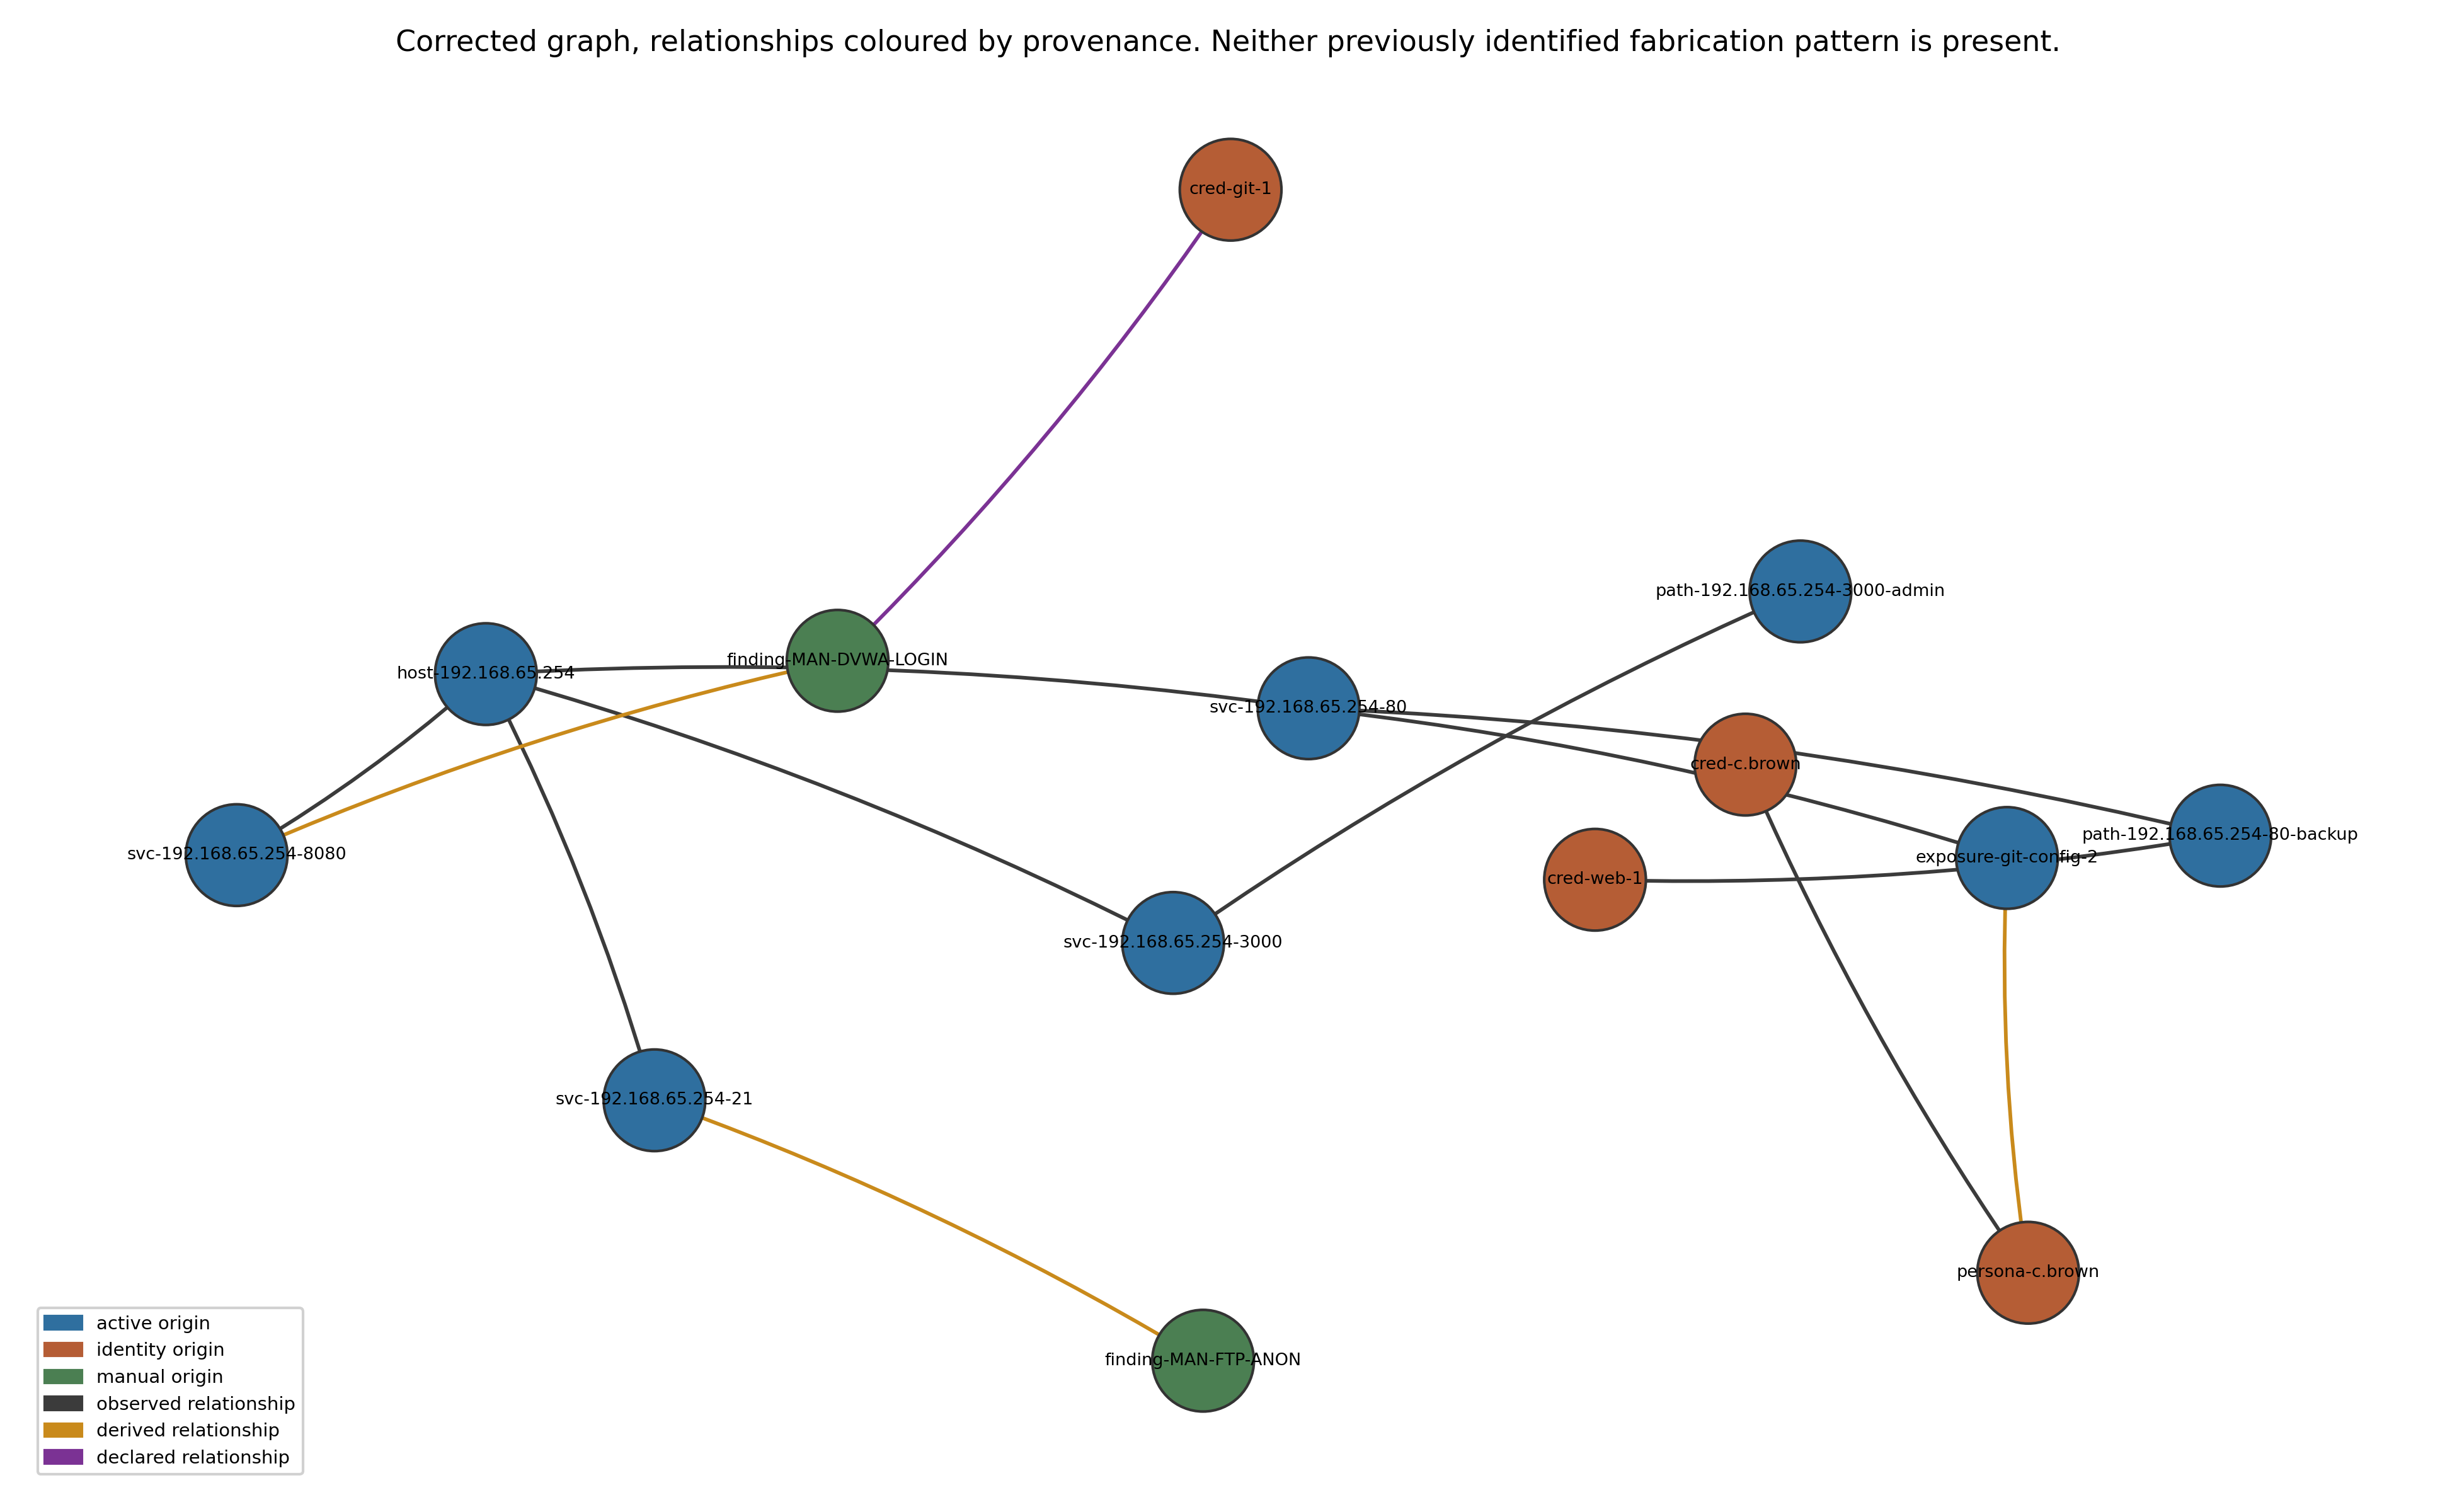
\includegraphics[width=0.95\textwidth]{out/derived_experiment_20260908/Figure_corrected_graph.png}
\caption{The corrected graph, edges coloured by provenance. No fabricated relationship
remains, and the credential recovered from the exposed backup directory and the exposure
identifying the persona are new, genuinely observed cross-layer evidence.}
\label{fig:corrected}
\end{figure}

\begin{figure}[H]
\centering
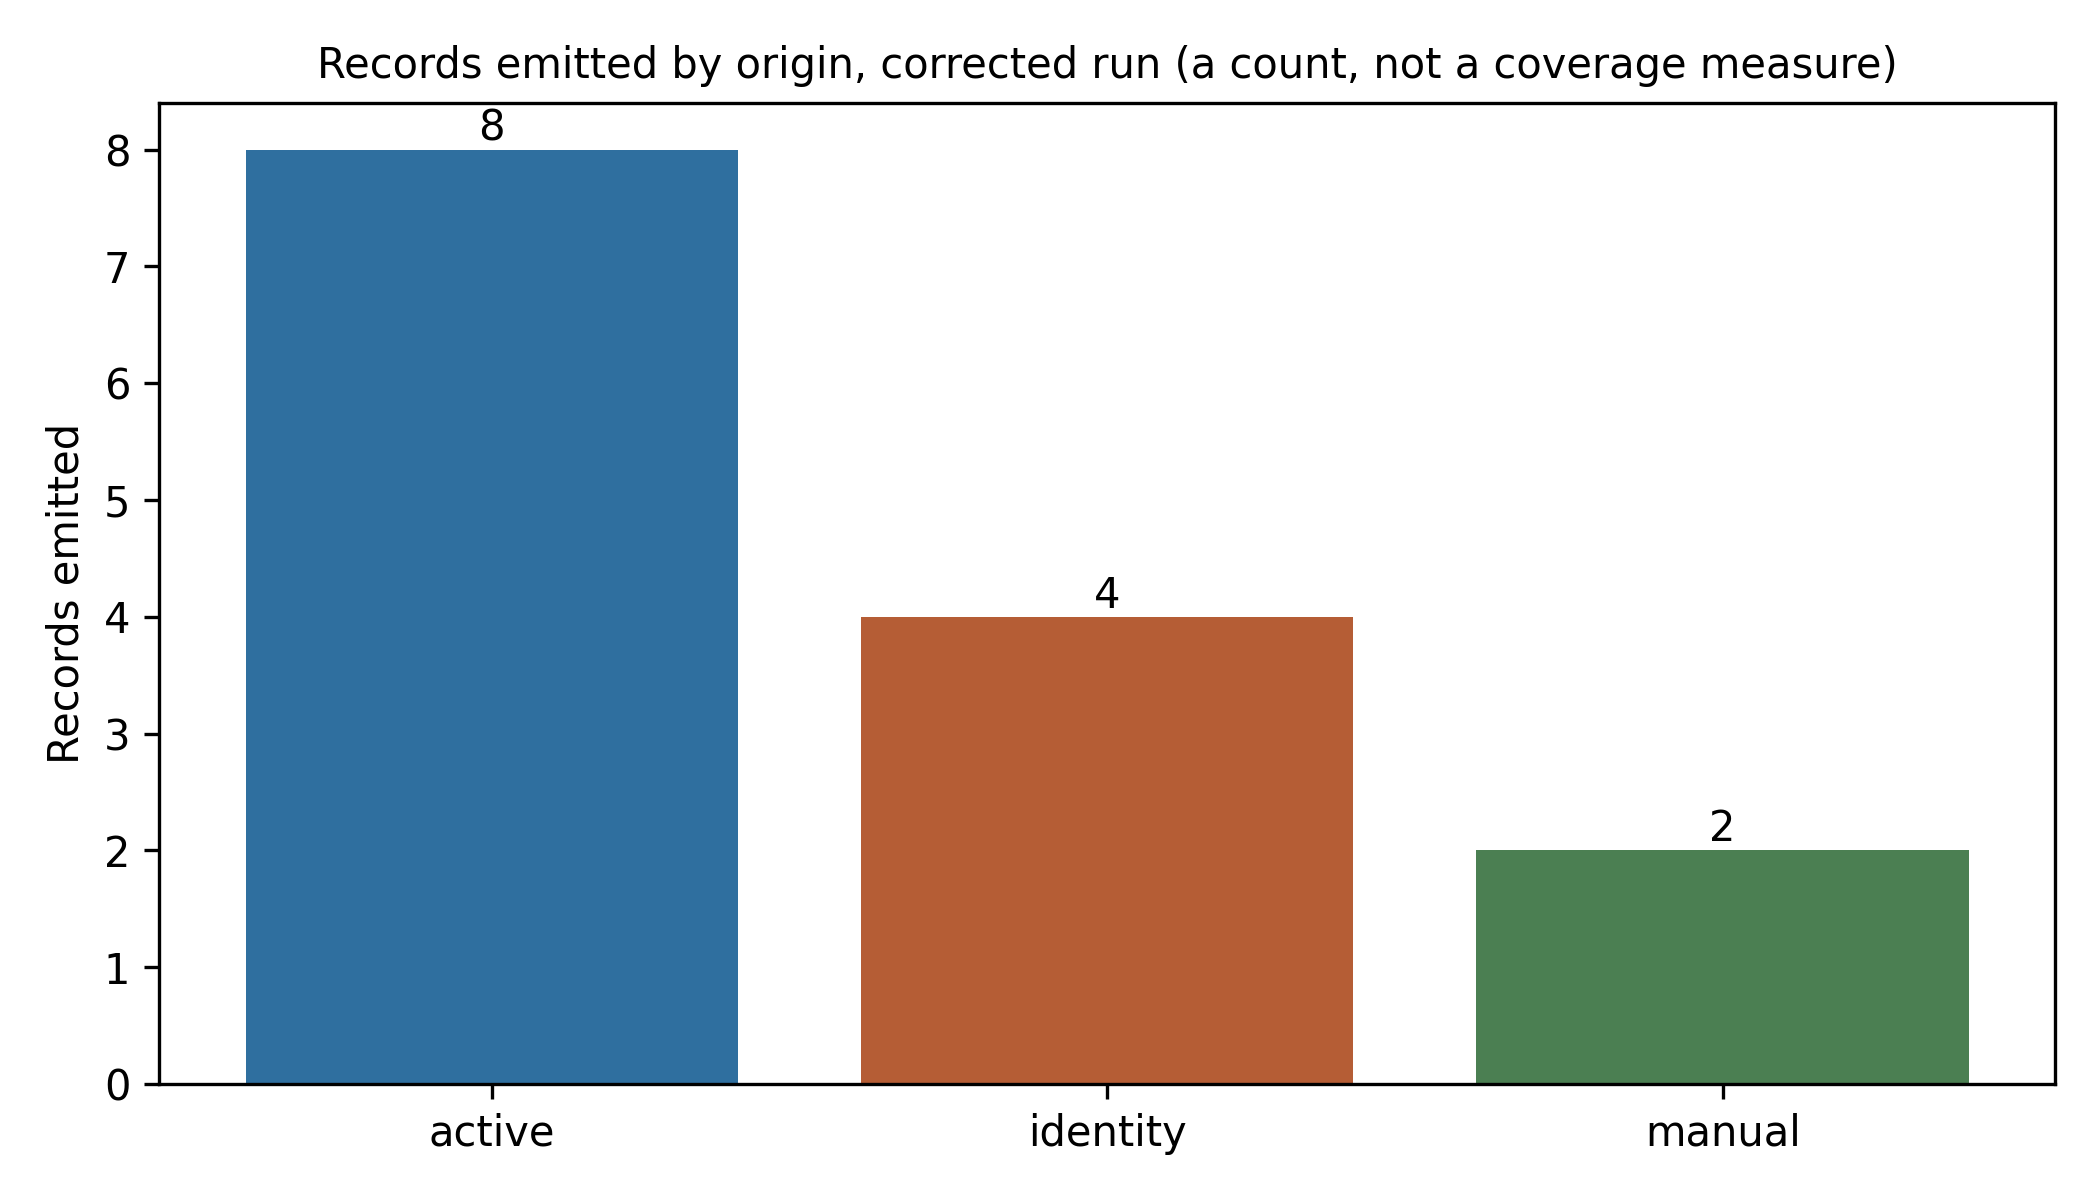
\includegraphics[width=0.62\textwidth]{out/derived_experiment_20260908/Figure_corrected_counts.png}
\caption{Records emitted by origin in the corrected run. This is a count of records, not a
coverage or recall measure.}
\label{fig:counts}
\end{figure}

\subsection{Ablation}
Table~\ref{tab:ablation} crosses collector subsets with provenance modes, reporting path counts under both traversal semantics.

\begin{table}[H]
\centering
\caption{Layer $\times$ provenance ablation on the corrected run. Attack traversal walks
capability edges only; evidence traversal walks all edge types. Every path count is zero.
The web-evidence rows drop one edge into the withheld identity stream, which is reported
rather than silently materialised as a node.}
\label{tab:ablation}
\small
\begin{tabular}{llrrcc}
\toprule
Layer subset & Provenance mode & Nodes & Edges & Attack paths & Evidence paths \\
\midrule
active only & observed-only & 7 & 6 & 0 & 0 \\
active only & derived & 7 & 6 & 0 & 0 \\
active only & all & 7 & 6 & 0 & 0 \\
\midrule
+ web evidence & observed-only & 9 & 8 & 0 & 0 \\
+ web evidence & derived & 9 & 8 & 0 & 0 \\
+ web evidence & all & 9 & 8 & 0 & 0 \\
\midrule
+ identity, secret & observed-only & 12 & 9 & 0 & 0 \\
+ identity, secret & derived & 12 & 10 & 0 & 0 \\
+ identity, secret & all & 12 & 10 & 0 & 0 \\
\midrule
+ manual (full) & observed-only & 14 & 9 & 0 & 0 \\
+ manual (full) & derived & 14 & 12 & 0 & 0 \\
+ manual (full) & all & 14 & 13 & 0 & 0 \\
\bottomrule
\end{tabular}
\end{table}

Reading across the provenance modes shows the three derivation rules contributing three edges and the analyst's declaration contributing one. Reading down shows each layer adding evidence. The path columns are zero throughout. We report zero because zero is what the corrected pipeline produces; we did not modify the testbed to obtain a positive result.

\subsection{Live End-to-End Confirmation}\label{sec:live}
The results above were first obtained by replay. To establish that they are not
an artifact of the replay fixtures, the complete pipeline was subsequently
executed end to end against the running testbed, writing to a separate directory
(\texttt{out/live\_run}). Active scanning, the bounded Nuclei scan, web-evidence
collection, identity collection, secret scanning and manual ingestion all ran
live; total runtime was 289\,s, dominated by exhaustive version probing.

The live run reproduces the replay result. Edge provenance is identical --- 9
observed, 3 derived, 1 declared --- as is the semantic composition: containment
6, evidence 4, validation 2, correlation 1, and \emph{no capability
relationship}. Attack traversal returns no path, and so does evidence traversal
under the three-origin predicate. Against the manifest the live run recovers all
five expected relationships and emits neither forbidden pattern. The graph
contains 17 nodes rather than 14 because the Nuclei collector completed in this
run and contributed three finding records, which the replay stream did not
contain; those records carry no outgoing relationships and do not affect any
path count.

The live execution also corrected an error in the replay fixtures, which we
record rather than quietly fix. The testbed's Nginx configuration defines two
name-based virtual hosts, and the exposed \texttt{.git/config} is served only
under the development name. A replay fixture had attributed that content to the
default virtual host, where the live server in fact returns 404. The
web-evidence collector now probes explicitly declared virtual host names
(\texttt{--vhost}), recording the name in the observation's source; under that
name the exposure is genuinely retrievable and the corresponding expected
relationship is recovered live. The fixture had asserted evidence at a location
that does not serve it --- the same class of defect this paper is about, found in
our own correction.

\subsection{Positive Control: A Live Capability Relationship}\label{sec:positive}
The evaluation to this point establishes only that the derivation rules decline
when evidence is absent. A rule that always declines would satisfy every result
reported so far. We therefore ran a separate live experiment, in a separate
output directory, to test whether the same rule emits a capability relationship
when the required evidence genuinely exists.

The conditions were established in a live Docker environment rather than by
replay. A Gitea 1.22.6 instance was running and reported version
\texttt{1.22.6} through its own API. A personal access token was issued by that
instance and verified against \texttt{/api/v1/user}, which returned the issuing
account; a deliberately incorrect token was rejected with HTTP 401. A repository
was configured with a remote addressing the running service, and a push through
that remote succeeded, establishing that the remote was functional rather than
decorative. The token was committed to the repository in the form a developer
would leave it, as a named assignment. The active collector then scanned the
environment independently and, because Nmap's version probe identifies this
service only as \texttt{Golang net/http server}, the product was established
from the service's own self-description captured by the \texttt{http-title}
script: \texttt{Gitea: Git with a cup of tea}.

Nothing in this arrangement tells the secret collector which service the
credential belongs to. The collector receives a repository path and the set of
observed services, and the relationship must follow from the conjunction of
remote, observation and credential compatibility.

It did. The rule emitted one capability relationship,
\begin{verbatim}
cred-git-1 --ENABLES_ACCESS [derived, conf 0.75]--> svc-10.41.159.81-3000
\end{verbatim}
with the justification: \emph{``repository remote
http://10.41.159.81:3000/pactest/pac-positive.git resolves to observed service
svc-10.41.159.81-3000 on port 3000; its observed http title is `Gitea: Git with
a cup of tea', which identifies product `gitea'; secret kind gitea-token
authenticates to that product''}. Attack traversal, restricted to capability
edges exactly as defined in Section~\ref{sec:semantics} and not relaxed,
returned one path, \texttt{cred-git-1} $\rightarrow$
\texttt{svc-10.41.159.81-3000}, with score $0.855$. By
Equation~\eqref{eq:path}: $0.75\times(0.9+0.3)\times0.95 = 0.855$. Under the
three-origin predicate used elsewhere in this paper the count is zero, because
this path spans two origins; the positive result concerns the emission of a
capability relationship and its acceptance by attack traversal, not the
three-origin predicate.

Two negative controls were run against the same live token and repository. With
the remote removed, the rule declined. With the remote present but the Gitea
observation withheld from the observed set, the rule declined. The only
difference between the positive and negative conditions is the presence of the
required evidence.

We checked that the result is independent of the original defect: neither
fabrication pattern is present in the source, every capability relationship in
the graph carries provenance \emph{derived}, no relationship was inserted
manually, and the token value appears in no artifact (the collector records the
secret's kind, commit and file, never its value).

\textbf{What this does and does not establish.} It establishes that the
corrected rule is capable of emitting a capability relationship, and that the
zero results reported elsewhere follow from absent evidence rather than from a
rule that cannot fire. It is a single controlled case in an environment we
constructed. It is not a measurement of accuracy, not evidence of generality or
production readiness, and carries no statistical weight.

\subsection{Tests}
The suite contains 74 tests, all passing. Thirty-five of them assert that a rule \emph{declines}, that a malformed input is \emph{rejected}, or that an identified defect \emph{cannot recur}. A repository with no remote yields no service edge. An incompatible secret kind yields none either. An uncorroborated username produces no account; a report naming an unobserved port produces no validation edge; an ambiguous host match is refused outright. An edge into an unemitted node is rejected, as is a derived edge carrying no justification. Declared edges are never promoted, and the two forbidden relationships stay absent from the recorded artifacts.

Tests shaped like that are the ones that would have caught the original defect. Of the eight present at the time, none was.

\section{Discussion}\label{sec:discussion}
\textbf{Confidence and provenance are orthogonal.} Confidence answers how strongly a relationship is asserted. Provenance answers where it came from and what evidential standing it has. The two vary independently --- a relationship can be weakly asserted yet directly observed, or carry a confident $0.75$ and be nothing more than a declaration. In the original schema both were collapsed onto a single numeric channel, with the consequence that a $0.75$ observed relationship and a $0.75$ declared relationship were evidentially equivalent to every downstream computation, and Equation~\eqref{eq:path} aggregated them identically. We do not claim this as a general theorem; we claim it as a design requirement supported by the failure documented here, namely that a system ranking paths over fused heterogeneous evidence should record both properties per edge if its output is to be interpretable.

\textbf{Semantics forms a third, separate axis.} Provenance alone would have been insufficient. A relationship may be directly observed and adequately justified and still not carry the meaning a traversal ascribes to it. The evidence chain scoring 1.354 illustrates this: two directly observed relationships, traversed as though they were attacker movement, outrank an unsupported relationship. We note again that this score arises under a relaxed two-origin predicate and is diagnostic of the traversal defect rather than a reported result of the corrected pipeline. Graph schemas in this setting should state, per edge type, whether a relationship expresses containment, evidence lineage, analyst validation, capability or unspecified association, and each traversal should declare which categories it is entitled to walk.

\textbf{On the objection that this is only an implementation error.} A hardcoded port constant is an ordinary coding defect, and we do not claim otherwise; nor do we claim this failure mode has not arisen elsewhere. The contribution is not the existence of the mistake but what it survived. Five conventional safeguards were in place and all of them passed: a confidence floor, a path-length penalty, a multi-origin predicate, exact score recomputation from stored artifacts, and a unit-test suite. None could detect the defect, because each operates downstream of graph construction and each takes the relationship as given. The architectural inference we draw is correspondingly narrow: relationship provenance and relationship semantics must be validated at the construction and traversal boundaries, because no downstream check over confidence values can recover information that construction discarded. We offer this as a design lesson supported by one documented case, not as a general theorem.

\textbf{Negative tests are the effective safeguard.} Part of why the defect persisted is that the test suite only ever checked that rules produced edges, never that they declined to. For an inference system whose characteristic failure is over-production, an assertion of absence carries more diagnostic weight than an assertion of presence. Thirty-five of the seventy-four tests in the corrected suite now take that form.

\textbf{Interpreting the zero result.} The corrected pipeline produced no valid attack path under the defined access-edge traversal semantics for this testbed. This does not establish that the testbed contains no attack path, and provides no evidence that the approach is incapable of finding one. It reflects a graph in which no capability relationship is currently derivable: the planted canary is inert and unassociated with any observed service, and no account was corroborated. An environment containing a credential that genuinely authenticates to an observed service would be expected to yield capability relationships and hence candidate paths; we did not modify the testbed to create one, because doing so would have manufactured the result. The defensible statement is narrower: the two paths previously reported do not survive either correction.

\textbf{Limitations.} These are listed individually rather than folded into a paragraph, because a summary would blunt them. Taken together they mean the results demonstrate regression and correction behaviour on a single controlled environment, and establish nothing about general recall or accuracy in any real setting.

\emph{Scale and setting.} The evaluation covers $n=1$ environment and $n=1$ configuration. The corrected results were obtained by replay and subsequently confirmed by one fresh live execution; there are no replicates of either.

\emph{Testbed.} A four-container synthetic environment with no production traffic, organizational noise or real identity owners. No result here generalizes to real infrastructure, and no evaluation in a real environment was performed.

\emph{Circular expectations.} The five expected relationships were intentionally planted, and the derivation rules were designed to recover them; both were authored by the same people, in an environment they constructed. The manifest therefore supplies regression criteria rather than independent ground truth. It guards against recurrence of the identified failure modes; it cannot detect a rule over-fitted to its own testbed, and the recovery figure must not be read as recall.

\emph{Absence of replicates.} There are no repeated runs, no independently labelled corpus, and consequently no detection-quality metrics and no inferential statistics.

\emph{Strength of the positive case.} The positive control of Section~\ref{sec:positive} is a single live instance, in an environment we constructed, exercising one derivation rule against one product. It shows the rule can fire on genuinely collected evidence; it does not measure how often it fires correctly, and it says nothing about credential or product types other than the one tested. The replay evaluation of Section~\ref{sec:eval} still contains no capability relationship of its own.

\emph{Rule dependence.} The derivation rules encode our judgement about what evidence implies. A different rule set yields a different graph, and we offer no argument that ours is optimal.

\emph{Heterogeneous edge direction.} The schema's edge directions do not express a single coherent relation: containment points from the contained entity to its container, evidence lineage from a fact to where it was found, and validation from a finding to the asset tested. We retained these directions and classified them rather than reversing any edge for algorithmic or visual convenience, which preserves fidelity to what each collector asserts at the cost of a graph in which direction carries no uniform meaning. A coherent directional ontology is future work and is not attempted here.

\emph{Scoring function.} Equations~\eqref{eq:cr} and~\eqref{eq:path}, their weights, $\lambda$, the confidence floor and the length bound are prototype conventions. They have not been validated as an objective measure of attack risk, and no such claim is made.

\textbf{On the positive control.} An earlier version of this work reported that the corrected attack traversal had never returned a non-empty result on collected data, and identified the corresponding live experiment as the most consequential gap in the evaluation. That experiment has since been performed and is reported in Section~\ref{sec:positive}. It required two capability additions that the attempt itself exposed: the active layer did not previously capture a service's self-description, so a product identifiable only by its own response could not be recognised; and the secret pattern for Gitea credentials did not match the unprefixed 40-character tokens the running version actually issues. Both were corrected, and both corrections are covered by tests. We did not plant a token or fabricate a remote in the replay testbed of Section~\ref{sec:eval}, whose results are unchanged.

\textbf{Reproducibility.} The corrected results were first produced by replay, with Docker unavailable, and we characterize that reconstruction precisely before describing the live confirmation. Its active-layer stream is the stream recorded by the earlier live run, relabelled with the provenance the current collector emits and otherwise byte-identical in content. Its web-evidence stream was collected in replay mode against response bodies taken verbatim from the testbed's own served files and from the recorded Nuclei response for the backup directory listing. The identity, secret and manual streams were regenerated by executing the current collectors against local fixtures. The derivation rules, endpoint validation, manifest check, ablation and scoring therefore ran on real recorded content, are deterministic given that content, and can be re-verified from the stored artifacts. What replay alone could not show is that a fresh collection against live containers yields the same streams. A live end-to-end execution has since shown exactly that (Section~\ref{sec:live}), reproducing the provenance composition, the semantic composition, the manifest outcome and every path count. Replay is no longer the sole basis for any reported result --- though the environment behind both runs is the same single controlled testbed, and that limitation is untouched by the confirmation.

\section{Conclusion}
A cross-layer security-evidence fusion prototype produced two ranked evidence paths under its original traversal semantics, the highest scoring 0.914. The scoring computation was internally consistent and exactly reproducible from the stored artifacts. Forensic analysis established that the relationships carrying that result were not independently evidence-supported: a fixed service target emitted for every repository credential, an analyst-supplied field converted directly into a graph relationship, and an account relationship generated from an email address alone. Every validation the system performed was satisfied, because each concerned how strongly a relationship was asserted and none concerned its evidentiary origin.

We separated three questions that the original schema conflated: how strongly a relationship is asserted (confidence), how it came to be known (provenance), and what it asserts about the world (semantics). The corrected implementation records all three, requires justification for derived relationships, allows derivation rules to decline, refuses edges into nodes no collector emitted, and restricts attack traversal to capability relationships. Against a manifest of controlled expectations it recovered all five expected relationships and emitted neither of the two previously identified fabrication patterns, and it produced no valid attack path under the defined access-edge traversal semantics in any configuration.

We report the zero result because it is what the evidence supports. The contribution is not a system that discovers attacks: the corrected pipeline discovered none, and the present testbed contains no capability relationship for it to discover. The contribution is a documented failure mode in security-evidence fusion, evidence that conventional safeguards did not detect it, and a construction discipline that prevented the identified patterns from recurring under controlled regression testing.

\appendix
\section{Artifact-to-Claim Ledger}
Every claim in this paper and the artifact supporting it. Baseline rows describe the
original result and are not presented as a correct reference.

\begin{longtable}{p{0.40\textwidth}p{0.54\textwidth}}
\caption{Claims and their evidence.}\label{tab:ledger}\\
\toprule Claim & Evidence \\
\midrule
\endfirsthead
\toprule Claim & Evidence \\
\midrule
\endhead
Baseline: 13 nodes, 13 edges, 2 paths, top 0.914 & \texttt{scripts/compare\_baseline\_corrected.py} over the stored baseline streams \\
Baseline top path's edges were hardcoded & \texttt{run\_secret\_scan.py} literal \texttt{svc-\{ip\}-3000}; \texttt{run\_manual.py} pass-through of \texttt{related\_credentials} \\
No FTP account for c.brown existed & \texttt{FTP\_USER=test} in \texttt{testbed/\bs docker-compose.yml} \\
Observed evidence chain scores 1.354 under all-edge traversal with a relaxed two-origin predicate (diagnostic, not a headline result) & \texttt{scripts/\bs verify\bs \_evidence\bs \_chain.py}; \texttt{out/\bs derived\bs \_experiment\bs \_20260908/\bs evidence\bs \_chain\bs \_scores.json} \\
Corrected: 14 nodes, 13 edges, 9/3/1 provenance & \texttt{out/\bs derived\bs \_experiment\bs \_20260908/\bs experiment\bs \_results\bs \_all.json} \\
Corrected graph has zero capability edges & \texttt{semantic\_counts} in the same result files \\
Zero paths in all modes, both traversals & \texttt{experiment\bs \_results\bs \_\{observed-only,\bs derived,\bs all\}.json} \\
All five expected relationships recovered; neither forbidden pattern emitted (controlled regression check, not a recall statistic) & \texttt{scripts/\bs run\_ablation.py} against \texttt{testbed/\bs seed\bs \_manifest.json} \\
74 tests pass, 35 of them negative & \texttt{python -m unittest discover -s tests} \\
Endpoint validation rejects phantoms & \texttt{tests/\bs test\_graph\_integrity.py} \\
Replay result confirmed by a fresh live end-to-end run & \texttt{out/\bs live\bs \_run/\bs experiment\bs \_results.json}; Section~\ref{sec:live} \\
\bottomrule
\end{longtable}

\section{References}\label{app:refs}
All entries were checked against publisher records or project documentation.
\begin{enumerate}[leftmargin=*,label={[\arabic*]}]
\item Sheyner, O.; Haines, J.; Jha, S.; Lippmann, R.; Wing, J.M. Automated Generation and Analysis of Attack Graphs. In \textit{Proc.\ IEEE Symposium on Security and Privacy}, 2002, pp.\ 273--284.
\item Ammann, P.; Wijesekera, D.; Kaushik, S. Scalable, Graph-Based Network Vulnerability Analysis. In \textit{Proc.\ 9th ACM Conference on Computer and Communications Security (CCS)}, 2002, pp.\ 217--224.
\item Ou, X.; Govindavajhala, S.; Appel, A.W. MulVAL: A Logic-Based Network Security Analyzer. In \textit{Proc.\ 14th USENIX Security Symposium}, 2005.
\item Ingols, K.; Lippmann, R.; Piwowarski, K. Practical Attack Graph Generation for Network Defense. In \textit{Proc.\ 22nd Annual Computer Security Applications Conference (ACSAC)}, 2006, pp.\ 121--130.
\item Mehta, V.; Bartzis, C.; Zhu, H.; Clarke, E.; Wing, J.M. Ranking Attack Graphs. In \textit{Recent Advances in Intrusion Detection (RAID 2006)}, LNCS 4219, Springer, 2006, pp.\ 127--144.
\item Wang, L.; Islam, T.; Long, T.; Singhal, A.; Jajodia, S. An Attack Graph-Based Probabilistic Security Metric. In \textit{Data and Applications Security XXII (DBSec 2008)}, LNCS 5094, Springer, 2008, pp.\ 283--296.
\item Manadhata, P.K.; Wing, J.M. An Attack Surface Metric. \textit{IEEE Transactions on Software Engineering}, 2011, 37(3), 371--386.
\item Durumeric, Z.; Wustrow, E.; Halderman, J.A. ZMap: Fast Internet-Wide Scanning and Its Security Applications. In \textit{Proc.\ 22nd USENIX Security Symposium}, 2013, pp.\ 605--620.
\item Lyon, G.F. \textit{Nmap Network Scanning: The Official Nmap Project Guide to Network Discovery and Security Scanning}. Nmap Project, 2009.
\item Yadav, A.; Kumar, A.; Singh, V. Open-source intelligence: a comprehensive review of the current state, applications and future perspectives in cyber security. \textit{Artificial Intelligence Review}, 2023, 56, 12407--12438. \url{https://doi.org/10.1007/s10462-023-10454-y}.
\item Babenko, T.; Kolesnikova, K.; Abramkina, O.; Vitulyova, Y. Automated OSINT Techniques for Digital Asset Discovery and Cyber Risk Assessment. \textit{Computers}, 2025, 14(10), 430. \url{https://doi.org/10.3390/computers14100430}.
\item Edwards, M.; Larson, R.; Green, B.; Rashid, A.; Baron, A. Panning for gold: automatically analysing online social engineering attack surfaces. \textit{Computers \& Security}, 2017, 69, 18--34.
\item Hagberg, A.; Schult, D.; Swart, P. Exploring Network Structure, Dynamics, and Function using NetworkX. In \textit{Proc.\ 7th Python in Science Conference (SciPy)}, 2008, pp.\ 11--15.
\item OWASP Foundation. \textit{Web Security Testing Guide}, version 4.2, 2020.
\item Penetration Testing Execution Standard (PTES). \url{http://www.pentest-standard.org}.
\item Dewhurst, R. Damn Vulnerable Web Application (DVWA). \url{https://github.com/digininja/DVWA}.
\item Sikos, L.F. Cybersecurity knowledge graphs. \textit{Knowledge and Information Systems}, 2023, 65, 3511--3531. \url{https://doi.org/10.1007/s10115-023-01860-3}.
\item Zhao, X.; Jiang, R.; Han, Y.; Li, A.; Peng, Z. A survey on cybersecurity knowledge graph construction. \textit{Computers \& Security}, 2024, 136, 103524. \url{https://doi.org/10.1016/j.cose.2023.103524}.
\item Zipperle, M.; Gottwalt, F.; Chang, E.; Dillon, T. Provenance-based Intrusion Detection Systems: A Survey. \textit{ACM Computing Surveys}, 2022, 55(7), Article 135. \url{https://doi.org/10.1145/3539605}.
\item Happe, A.; Cito, J. Benchmarking Practices in LLM-driven Offensive Security: Testbeds, Metrics, and Experiment Design. \textit{arXiv preprint} arXiv:2504.10112, 2025. \url{https://arxiv.org/abs/2504.10112}.
\end{enumerate}

\end{document}
